\part{Fejlesztői dokumentáció}

\section{Felhasznált technológiák}
A fejlesztés során fejlesztőkörnyezetet használtam, így viszonylag sok probléma már a fordítás és futtatás előtt kiderült. Ahogy korábban is leírtam, a programcsomagnak szüksége van MySQL Serverre az adatbázis kérdése miatt. A kódot verziókkal is el kellett látnom, így egy verziókezelő rendszert is felhasználtam. Az osztály- és moduldiagramok szerkesztésére ugyancsak külső szoftvercsomagot használtam fel. A programcsomag több modulból épül fel, ezért ugyancsak szükségessé vált egy buildrendszer használata, amely a modulok közötti függőségek kezeléséért felelős.

\subsection{Eclipse}
A szakdolgozatom eclipse Mars \cite{eclipse_mars} fejlesztőkörnyezetben írtam, amelyhez a quick search \cite{quick_search} nevű plugint is letöltöttem. A fejlesztést nagy mértékben megkönnyítette a fejlesztőkörnyezet használata, ugyanis többek között szintaktikus és classpath ellenőrzést is végzett. Továbbá remekül paraméterezhető jóformán tetszőleges billentyűkombinációkkal.

\subsection{Maven}
A népszerű buildrendszerből a 3.3.3-as verziót használtam, amelyhez igen sok különböző plugin szerezhető be. Eredetileg csupán a függőségek kezelésére alkalmaztam volna a programot, később egyre több és több pluginnal egészítettem ki, így egyre több feladatot volt képes ellátni a szoftver.

\pokerparagraph{Adatbázis séma létrehozása és demó adatokkal való feltöltése}
Az adatbázis sémát a fejlesztés elején mindig manuálisan készítettem el, majd rátaláltam a sql-maven-plugin nevezetű pluginra. A maven honlapján megtalálható teljeskörű dokumentáció segítségével bekonfiguráltam a plugint, így csupán a
 \begin{verbatim}
mvn sql:execute@create-db
mvn sql:execute@create-triggers
mvn sql:execute@fill-db
\end{verbatim}
utasításokat kellett kiadnom parancssorból, hogy friss adatbázissal dolgozhassam tovább. A felesleges parancsismétlések elkerülése végett letöltöttem az exec-maven-plugin nevű plugint, amelynek segítségével sikerült a 
 \begin{verbatim}
mvn exec:exec
\end{verbatim}
parancsra korlátozni az adatbázis újboli létrehozását. A feladatot tovább általánosítottam, majd végül egy profilt készítettem el, amely az install fázissal együtt oldja meg az adatbázis kérdését. A 
 \begin{verbatim}
 mvn clean install -Pbootstrap
 \end{verbatim}
paranccsal nem csak a lokális repozitorinkba telepíthetjük fel a poker-persist modult, de még egy új adatbázist is kapunk.

\pokerparagraph{Javadoc}
A mavennel java dokumentációt is lehet generáltatni. Navigáljunk a poker könyvtárba és adjuk ki a
\begin{verbatim}
 mvn javadoc:javadoc
\end{verbatim}
 parancsot. Aggregált java dokumentációra is lehetőség van a 
 \begin{verbatim}
 mvn javadoc:aggregate
\end{verbatim}
 Sőt, akár modul dokumentációt is lehet készíteni a 
\begin{verbatim}
 mvn site:site
 mvn site:stage
\end{verbatim}
utasításokkal. Az elkészült dokumentációk a modul \path{poker\target\staging} könyvtárba kerülnek. Kettő darab index.html állományt kell keresnünk, az egyik a gyökérkönyvtárban található a másik pedig az \path{apidocs} könyvtár gyökerében.
 
\subsection{MySQL}
Az adatok perzisztens tárolásáért egyértelműen relációs adatbázisra volt szükség. A MySQL adatbázissal már korábban is találkoztam, ismert technológiát szerettem volna flehasználni.

\subsection{Git}
A fejlesztés során előfordult, hogy internet kapcsolat nélkül kellett verzióznom a kódomat. A git egyik legnagyobb előnye, hogy internet kapcsolat nélkül is lehet commit parancsot végrehajtani. A commit parancs hatására a lokális repozitorinkba egy új pillanatfelvétel készül az aktuális munkakönyvtárunk tartalmáról, amelyet később push utasítással feltölthetünk egy távoli repozitoriba. A fejlesztéshez több branchet is használtam, így ha valami balul sült volna el, akkor egyszerűen visszaálltam volna a masterre.

\subsection{Enterprise Architect}
A tervezés során igen nagy hasznát vettem ennek a szoftvernek. Rengeteg beállítás, funkció megtalálható a programban. Szinte minden testreszabható az UML diagramokat érintő kérdések körében. Az elkészült UML diagramokból pedig JAVA kódot tud generálni a program. A dokumentációban fellelhető osztály hiearchiák és UML diagramok ennek a szoftvernek a segítségével készültek el.

\section{Adatbázis séma}
\begin{figure}[h!]
  \caption{Adatbázis séma}
  \label{fig:db_scheme}
  \centering
    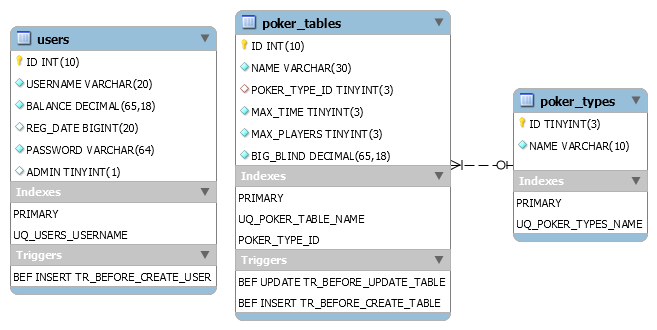
\includegraphics[width=\textwidth]{user-documentation/images/db_scheme2.png}
\end{figure}
Az adatbázis három darab táblából épül fel, amelyet a \ref{fig:db_scheme}. ábra szemléltet.

\subsection{Póker játék asztal tábla}
\begin{tabular}{| C{4.7cm} | C{4.7cm} | C{4.7cm} |}
\hline
  \thead{Oszlopnév} & \thead{Típus} & \thead{Megszorítás} \\ \hline
  ID & UNSIGNED INT & Elsődleges kulcs a táblára nézve. \\ \hline
  NAME & VARCHAR & Az oszlopban szereplő értékeknek egyedinek kell lenniük és legfeljebb 30 karakter hosszúak lehetnek.  \\ \hline
  POKER\_TYPE\_ID & UNSIGNED TINYINT & Az oszlop idegen kulcs a poker\_types táblára nézve. \\ \hline
  MAX\_TIME & UNSIGNED TINYINT & Az értéknek bele kell esnie a [5-40] intervallumba. \\ \hline
  MAX\_PLAYERS & UNSIGNED TINYINT & Az értéknek bele kelle esnie a [2-5] intervallumba. \\ \hline
  BIG\_BLIND & DECIMAL & - \\ \hline
\end{tabular}

\subsection{Felhasználók tábla}
\begin{tabular}{| C{4.7cm} | C{4.7cm} | C{4.7cm} |}
\hline
  \thead{Oszlopnév} & \thead{Típus} & \thead{Megszorítás} \\ \hline
  ID & UNSIGNED INT & Elsődleges kulcs a táblára nézve. \\ \hline
  USERNAME & VARCHAR & Az oszlopban szereplő értékeknek egyedinek kell lenniük és legfeljebb 20 karakter hosszúak lehetnek.  \\ \hline
  BALANCE & DECIMAL & - \\ \hline
  REG\_DATE & BIGINT & - \\ \hline
  PASSWORD & VARCHAR & Az értéknek pontosan 64 hosszúnak kell lennie. \\ \hline
  ADMIN & UNSIGNED TINYINT & Az érték csak 0 vagy 1 lehet. \\ \hline
\end{tabular}

\subsection{Játékstílus tábla}
\begin{tabular}{| C{4.7cm} | C{4.7cm} | C{4.7cm} |}
\hline
  \thead{Oszlopnév} & \thead{Típus} & \thead{Megszorítás} \\ \hline
  ID & UNSIGNED INT & Elsődleges kulcs a táblára nézve. \\ \hline
  NAME & VARCHAR & Az oszlopban szereplő értékeknek egyedinek kell lenniük és legfeljebb 10 karakter hosszúak lehetnek.  \\ \hline
\end{tabular}

%\begin{itemize}[leftmargin=2.7cm]
%\item users
%\item poker\_tables
%\item poker\_types
%\end{itemize}



\hfill \break
Minden tábla rendelkezik elsődleges kulccsal, amelynek típusait a fentebb látható táblázat tartalmazza. A \texttt{poker\_types} tábla elsődleges kulcsa UNSIGNED TINYINT, melyet a MySQL Server 4 byteon tárol. Az adatábrázolás mértékének a szűkítése ebben az esetben indokolt, ugyanis a 255 különböző értékű UNSIGNED TINYINT típus kielégíti a játéktípusok által támasztott követelményeket. \\
Az adatbázis sémában három darab trigger van definiálva:
\begin{itemize}
\item Tábla beszúrás előtti
\item Tábla módosítás előtti
\item Felhasználó beszúrás előtti
\end{itemize}


%A játékstílusok neveit is el kell tárolni, amelynek a maximális hossza 10 karakterben lett meghatározva, amely triggerrel van védve. A users tábla tartalmazza a regisztrált felhasználókat. A regisztrált felhasználók felhasználónévvel és jelszó párossal tudnak regisztrálni, és ennek megfelelően ezek az adatok tárolásra is kerülnek. A felhasználónév maximális hossza 20 karakter, ameyelet triggerrel ellenőrzök. A jelszót bcrypt függvénnyel nyírom. Só eltárolása nem szükséges a bcrypt implementációjából adódóan. A felhasználóról el kell még tárolni a regisztráció dátumat, amely a szerver ideje alapján számolódik és UNIX timestampként kerül letárolásra, továbbá a jogosultsági (admin) szintet, amely ugyancsak 4 byteon (TINYINT) kerül ábrázolásra. A 0/1 értékek megfeleltethetőek a TRUE/FALSE logikai típusú konstans értékeknek, így tehát, ha az érték 0, vagyis FALSE, akkor az adott felhasználó nem rendelkezik admin jogkörrel, különben igen. Ugyancsak tárolandó érték a felhasználó játékbeli egyenlege, amely BIGDECIMAL típúsként van ábrázolva.
%A játéktáblákat a poker\_tables adatbázis tábla tárolja. Szükségünk van eltárolni a játéktábla nevét, melynek felső korlátja 30 karakter és egyedinek kell lennie. Ezeket a megszorításokat szintén triggerekkel ellenőrzöm. A játék asztal játékstílusát is eltárolom, amely egyben idegenkulcs is a poker\_types táblára nézve. Továbbá minden asztal tulajdonsága, hogy maximum hányan játszhatnak rajta, és hány másodpercig gondolkodhatnak a játékosok. Ezen két érték típusaként ugyancsak UNSIGNED TINYINT van meghatározva, ugyanis az egyes asztaloknál a játékosok száma legfeljebb 5 lehet, míg az egyes játékosok gondolkodási ideje maximum 40, de legalább 5 másodperc.

\section{Megoldási terv}
\subsection{Probléma}
Egy hálózaton keresztül működő póker játékot szolgáltató kliens-szerver programcsomagot fogok megvalósítani JAVA programozási nyelven. A felhasználói és szolgáltatással kapcsolatos adatokat egy adatbázisban helyezem el, így is biztosítva a játék menet konzisztenciáját és konkurencia vezérlését. Az említett adatabázis többek között rögzíti az olyan profil adatokat, mint a felhasználói név, a jelszó vagy a regisztráció dátuma.
Az alkalmazás szerver-oldali komponensei több olyan asztal szimultán futtatását biztosítja, amelyek különböző paraméterezésűek lehetnek. Ugyanis felhasználói oldalról különböző igények léphetnek fel (pl.: a tapasztaltabb játékosok rövidebb idő alatt tudnak reagálni egy leosztásra). Az asztalok leglényegesebb paraméterei a játék stílus, a játék gyorsasága, illetve az elfoglalható helyek száma lesz, de ezeken felül további paraméterek is megadhatóak egy konkrét asztal instancia létrehozásakor. Ezen műveletek ellátására, azaz az asztalok konfigurálására, egy grafikus interfészt valósít meg a programcsomag. \\
A játékban a felhasználók jogok alapján is megkülönböztethetőek lesznek, így a magasabb jogkörrel rendelkező felhasználók speciális műveleteket hajthatnak végre a játékon és az adatbázison egyaránt. Ebből kifolyólag külön adminisztrációs felület is megvalósításra kerül majd, amelyen keresztül adott esetben akár rendezni (név, regisztráció dátuma, stb. alapján), ill. törölni is lehet majd felhasználókat, sőt a különböző felhasználóknak különböző jogokat is itt lehet majd kiosztani. Továbbá a felhasználók könnyen tudják majd menedzselni a saját felhasználói fiókjukat, ugyancsak egy grafikus interfész segítségével.

\subsection{Tervezés}
A probléma leírásából fakadóan egyértelműen kiderül, hogy legalább kettő darab modulra lesz szükségünk, egy kliens modulra és egy szerver modulra. 
A tervezés során végig kellett gondolni, hogy mik azok az igen fontos események amelyek a program futása során bekövetkeznek, illetve bekövetkezhetnek. A szerver és a kliens hálózaton keresztül fognak kommunikálni, így kínálkozik a lehetőség az RMI architektúrára való építkezésre. Ha RMI, akkor egy jóldefiniált publikus interfészt kell elkészíteni, amely a szerver vázáért felel. A kliensek ezen az interfészen keresztül hívnak be a szerverhez. A probléma megfogalmazásából kiderül, hogy melyek azok az alapvető funkciók és szolgáltatások, amelyeket a szervernek biztosítania kell. Ezen megfogalmazás alapján már körvonalazódik a szerver modul feladata. A probléma leírásából a szerver és a kliens között kiépített kommunikációs rendszer csak implicit megfogalmazásban szerepel. Az, hogy hogyan és miként, illetőleg milyen szekvencia szerint fognak egymással kommunikálni a modulok az explicite nincs felvázolva. Az implementáció során ügyelni kell arra is, hogy párhuzamosan akár több kliens is csatlakozhatva lehet a szerverhez, illetve az egyes játék asztalokhoz. Az üzenetek egy előre meghatározott sorrend alapján küldhetőek és fogadhatóak. Fontos megjegyezni, hogy nem csak a kliensek küldhetnek üzeneteket a szervernek, hanem a szerver is értesítheti a klienseket a szerveren történő eseményekről, mint például, ha egy adott asztalnál egy játékos CALL utasítást küld a szervernek, akkor a szerver az asztalnál ülő játékosokat értesíti a bekövetkezett eseményről. Ennek megfelelően a kliensek mindig értesítést kapnak az őket érintő eseményekről. Ezáltal a kliens modulnak is meg kell fogalmazni egy publikus interfészt, amelyet a szerver fog felhasználni. Fontos megjegyezni, hogy a kliensek közvetlenül egymásnak nem küldhetnek üzeneteket. A szervert úgy kell implementálni, hogy a béerkező üzenetek alapján az összes megfelelő klienst értesítse. \\
Az üzeneteknek kettő fajtáját különböztetjük meg
 \begin{itemize}[leftmargin=2.7cm]
\item Szerver által küldött üzenet
\item Kliens által küldött üzenet
\end{itemize}
A megfelelő absztrakció elérése érdekében a \ref{fig:messaging}. ábrán látható \texttt{PokerCommand} interfésszel össze kell fogni az üzenet fajtákat.
\begin{figure}[h!]
	\caption{Póker üzenetek felépítése}
	\label{fig:messaging}
	\centering
	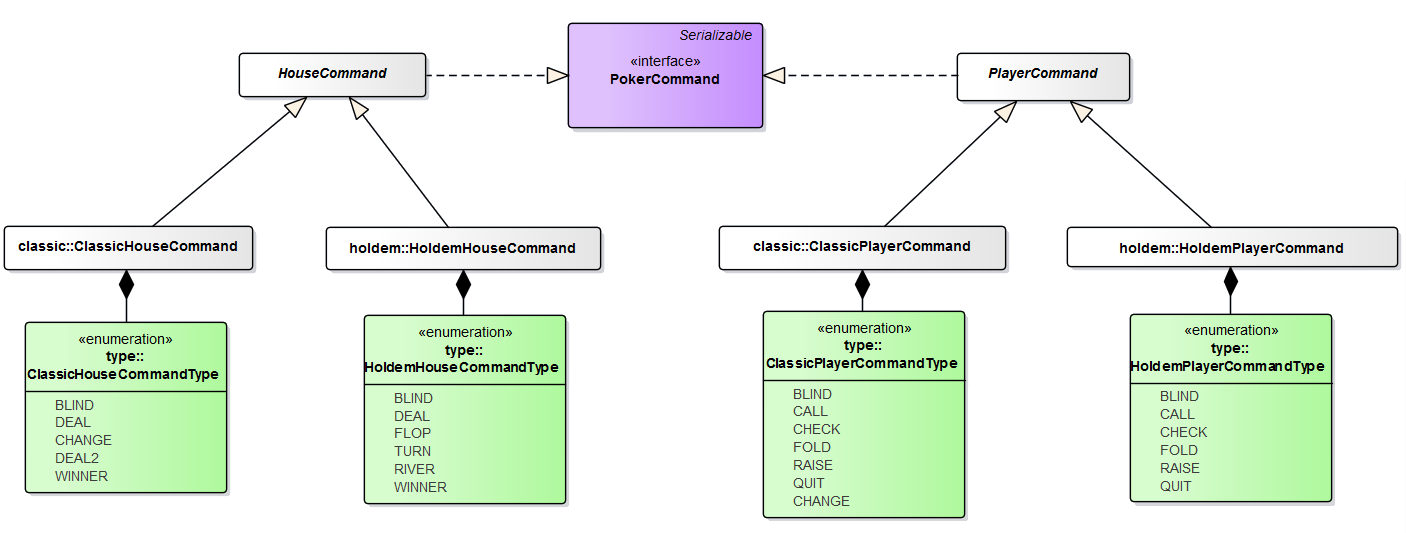
\includegraphics[width=\linewidth]{developer-documentation/images/messaging.png}
\end{figure}
A \ref{fig:messaging}. ábráról leolvasható, hogy minden üzenetnek van egy típusa. Az üzenet típusa függ az üzenet fajtájától és specializációjától is. Például ha egy Texas Hold'Em játékstílusú asztal be szeretné kérni a vakokat a játékosoktól, akkor egy \texttt{HoldemHouseCommand} típusú \texttt{HoldemHouseCommandType::BLIND} utasítástípusú új objektum példányt kell szétküldenie az asztalnál ülő összes játékosnak. Ezt az üzenetküldést a szerver a kliensek publikus interfészén keresztül teheti meg. \\
A kliensnek az üzenetet fogadnia kell. Az üzenet fogadására egy új, ezt a funkciót ellátó objektumot kell definiálni. \\
A kliens oldal architektúrális felépítésének az alapját a Model-View-Controller tervezési minta adja. A beérkezett üzenetet az erre kijelölt objektum fogadja, majd továbbítja a kliens oldali vezérlő rétegnek. A vezérlő réteg értelmezi a bejövő üzenetet, majd ennek megfelelően a model rétegnek és a megjelenítési rétegnek is továbbítja a beérkezett üzenetet további feldolgozásra. A probléma különböző funkciók leírását is tartalmazza. Célszerű, hogy a különböző funkcióknak különböző grafikus interfészt biztosítsunk. Ugyanakkor új felület létrehozásakor új vezérlő objektumot is létre kell hoznunk, viszont a model rétegnek statikusnak kell lennie. Ugyanaz a model objektum lássa el például a bejelentkezési és regisztrációs kérelmeknek a továbbítását a szerver felé. Tehát különböző funkciók elérése esetén a vezérlési és megjelenítési réteget ki kell cserélni, viszont a modelt nem. Illetőleg kettő darab modelt kell megfogalmaznunk, az egyik látja el például a fentebb említett egyszerűbb funkciók meghívását a szerveren, a másik pedig a tényleges játék közbeni model, amelyet a vezérlői réteg értesíteni tud a beérkezett üzenetekkel kapcsolatban és kliens oldalon biztosítja a játék menetet.  \\
A probléma leírásában szerepel adatbázissal való kommunikáció is. Erre ugyancsak egy új modult kell bevezetni, amely az adatbázissal történő kommunikációt bonyolítja le. Entitás osztályokat írni és olvasni kell az adtbázisból, így ezeket az osztályokat általánosan kell megfogalmazni a kód duplikációk elkerülése végett. Ezen modul vázlatát a \ref{fig:persist}. ábra szemlélteti. \\
\begin{figure}[h!]
	\caption{Az adatbázissal kommunikáló modul}
	\label{fig:persist}
	\centering
	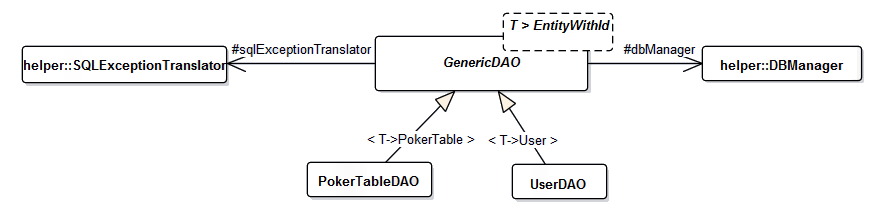
\includegraphics[width=\linewidth]{developer-documentation/images/dao.png}
\end{figure}
Az adatbázissal való kommunikációért felelős modul nem csak entitásokat tartalmaz, hanem további kettő darab objektumra is szükség lesz. Az \texttt{SQLExceptionTranslator} fontos része a modulnak. Az adatbázis triggerek és megszorítások által definiált hibaüzeneteket fordítja át JAVA kivételobjektumokra, amelyek a kódbeli feldolgozást könnyítik meg, továbbá ezek a saját kivételobjektumok már a felhasználó számára is értelmes hibaüzenetekkel bírnak. A \texttt{DBManager} osztály felelős az adatbázissal kiépített kapcsolat fenntartásáért és lezárásáért. \\
A szervernek szerves része egy objektum, amely a munkamenetek kezeléséért felelős. Az autentikált felhasználók egy-egy munkamenettel azonosíthatóak. Az autentikációért felelős részmodult a \ref{fig:sessionservice}. ábra vázolja fel.
\begin{figure}[h!]
	\caption{A munkamenetek tárolása szerver szinten}
	\label{fig:sessionservice}
	\centering
	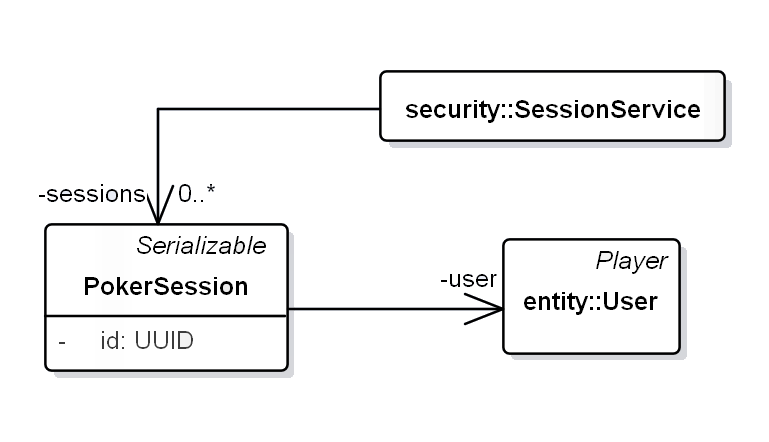
\includegraphics[width=\linewidth]{developer-documentation/images/session.png}
\end{figure}
A \texttt{SessionService} tartja nyilván a munkameneteket. Egy felhasználóhoz legfeljebb egy munkamenet rendelhető egy adott időben. Továbbá egy munkamenethez pontosan egy felhasználó tartozik. Ha a felhasználó kijelentkezik a póker játékból, akkor a felhasználó munkamenetét érvényteleníteni kell. Ugyanaz a munkamenet többször nem osztható ki, törölni kell. Ugyanakkor egy felhasználó különböző időpillanatokban rendelkezhet különböző munkamenetekkel. Tehát ha az imént kijelentkezett felhasználó újból be szeretne jelentkezni a játékba, akkor egy új munkamenettel kell azonosítani. A szervernek biztosítania kell, hogy a kliensek rendelkezzenek munkamenet objektumokkal, ugyanis bármilyen funkció hívása esetén a kliensek ezzel az objektummal azonosítják magukat. Pontosabban fogalmazva minden munkamenet egy-egy UUID értékkel van ellátva, és a klienseknek elég csak ezt az egyedi értéket elküldeni a szervernek. A felhasználóknak nem engedhetjük meg, hogy egy felhasználónevet konkurensen használhassanak. Ez a felügyelet ugyancsak a \texttt{SessionService} objektum feladata. \\
A szerver és a kliens közötti bárminemű tevékenység, illetve kommunikáció egy közös modult kell, hogy felhasználjon. Például ha kivételobjektumot szeretnénk dobni szerver oldalon és azt kliens oldalon szeretnénk lekezelni, akkor értelemszerűen mind szerver mind a kliens classpathján szerepelnie kell az adott kivételobjektumnak. A közös modulban kell szerepelnie a szerver és a kliens publikus interfészeknek, a kommunikációs rendszert alkotó osztályok összessége és a saját kivételosztályok definíciói. \\
Külön modul fogalmazható meg a játékosok lapjainak a kiértékelésére is. Ez a modul nem kerül implementálásra, külső könyvtárként kerül felhasználásra.

\subsection{Implementálás}
Az implementálást a kliens oldali megjelenítéssel kezdtem egy maven archetype generator segítségével. Így generálódott egy megfelelő kiindulási alap, amiből elkezdtem építkezni. Legelőször a bejelentkezési és a regisztrációs formot állítottam össze. Ezekután pedig a szerver publikus interfészének egy részét fogalmaztam meg kód szinten. Ezt az interfészt a kliens már el tudta kérni az RMI registry-ből \cite{RMI}, és sikeresen be tudott hívni a szerverhez. A szerver és a kliens kommunikációjának az alapjának a kiépítése után az adatbázis feltelepítése, elindítása majd elérése volt a legfőbb célom. \\
Miután sikerült promptból becsatlakoznom a MySQL Serverre, azután manuálisan létrehoztam egy kezdetleges adatbázis sémát és néhány egyszerű INSERT műveletet hajtottam végre az adatbázison. A kezdetleges demó adatokat a szerver oldali kóddal \texttt{PreparedStatement} objektumok segítségével olvastam ki. Ugyanezen objektumok segítségével írtam az adatbázisba. A későbbiek során kialakult a jóformán végleges adatbázis séma, amelyet egy sql állományban tároltam el, és ezt az állományt pusztán alkalmazni kellett az adatbázisra, ha új adatbázis sémát szerettem volna elérni. A későbbiek során az adatbázisba letárolt értékekre megszorításokat kellett alkalmaznom, amelyet akár triggerekkel, akár constraintekkel valósítok meg. Így az adatbázis sémát generáló sql állomány mellé létre kellett hoznom egy olyan sql állományt, amely triggereket aggat a meglévő adatbázisbeli adattáblákra. Továbbá a fejlesztés haladtával demó adatokat is kellett biztosítanom az adatbázis számára, ezzel is lerövidítve a fejlesztési időt. \\
Miután a szerver már képes volt az adatbázissal való kommunikációra, azután a már meglévő sql kódok és a tervezési fázisban felvázoltak alapján a poker-model modult el lehetett készíteni. Szükség volt egy közös interfészre, amely összefogja az entitásokat. Az interfész alapján el lehetett készíteni a \texttt{GenericDAO} osztályt, amely típusparaméterrel van ellátva. A típusparaméterre vonatkozó kritérium, hogy az \texttt{EntityWithId} interfészt implementálnia kell a paraméterül adott típusnak. A poker-persist modulnak rendelkeznie kell egy kapcsolatkezelő objektummal is. Ennek megvalósítása nem jelentett különösebb gondot, viszont a kapcsolat paraméterezésére utólag került sor. A már megírt triggerek alapján az \texttt{SQLExceptionTranslator} osztály implementációja ugyancsak könnyűnek mondható. A tervezett 6 darab modulból 2 darab már implementálásra került. \\
Mivel a szerver és a kliens közötti kapcsolat kiépítésre került, továbbá a szerver már az adatbázist is eléri, ezért a felhasználók bejelentkezése és regisztrációja következett. Ezen funkciók lefejlesztése után a további funkciók kerültek implementálásra. Többek között a játékasztal entitások létrehozása, módosítása, már meglévő felhasználók jelszavának módosítása, felhasználók törlése, adminisztrációs jogok kezelése. \\
A fejlesztési folyamat itt erősen megakadt, ugyanis nem tartottam egyszerűnek a tényleges póker játék szerverek implementációját, és a hozzájuk tartozó kliens oldali kód megírását. Így a már meglévő funkciókat kezdtem el tesztelni és tovább fejleszteni. Lefejlesztésre került a \texttt{SessionService} osztály is, amely a kliensek munkameneteinek kezeléséért felel. A fejlesztés korai fázisában volt egy hetedik, poker-security modul, amely a kliensek autentikálását és autorizációját végezte volna. Azonban a fejlesztés előrehaladtával és a kód refaktorálásával a modult fel kellett számolni és a modul végül egyetlen osztályként szerepel a poker-server modulban. \\
Az eddigi lefejlesztett funkciókon további fejlesztési lehetőség nem kínálkozott a tervezési fázisban megfogalmazottak alapján. A póker játék asztal szerverek implementációja következett. Legelőször a kliens oldali grafikus interfészt fejlesztettem le. Viszonylag hamar rá kellett jönnöm, hogy szükségem lesz egy olyan osztályra, amely a játék és a grafikus felület konstans értékeit szolgáltatja. Az fxml állományok nem kerülnek kifordításra, így ha módosítani kellett őket, akkor nem kellett a futó programot újraindítani, elég volt az adott fxml állományt újra betölteni, és a változások érvénybe léptek, így a fejlesztés ugyancsak felgyorsult. A póker asztalok pontos működésének a megfogalmazása és implementálása volt az első olyan pont a fejlesztés során, amelyet többször át kellett dolgoznom. A tervezési fázisban felváltoztak kód szinten közel sem triviálisnak mondható dolgok. A póker játék szerver implementálása során absztrakciós szintre nem gondoltam, így először minden a Texas Hold'Em játékstílus követelményei alapján került implementálásra. Ezután egy refaktorálás oldotta meg a fejlesztési fázis továbblépését, mind szerver, mind kliens oldalon. A refaktorálással és a hiányos tervezéssel viszonylag sok idő elúszott, pláne a Test Driven Development megközelítés mellőzése miatt is. Az eddig implementált funkciókat és működésbeli viselkedéseket refaktorálás után és közben folyamatosan manuálisan kellett tesztelni. \\
A refaktorálást követően nekiállhattam a klasszikus játékstílus implementálásának. Az implementálás során további osztályok absztrakciójára volt szükségem, így még több refaktorálást kellett elvégeznem a kódbázison. A refaktorálást követően a kódbázis sokkal letisztultabbá vált. Ugyanakkor az utasítások típusait enum objektumokként definiáltam, így az utasításokat nem tudtam kellően általánosan megfogalmazni. Később az utasítások típusait egy interfésszel összefogtam, majd a \texttt{GenericDAO} mintájára típusparaméterrel láttam el a \texttt{PokerCommand} interfészt. A megközelítés sikertelenül zárult. A típusparamétert eggyel lejjebbi szintre süllyesztettem, tehát a következőkben a \texttt{HouseCommand} és \texttt{PlayerCommand} osztálydefiníciókat láttam el típusparaméterrel, és az utasítások típusait másmilyen formában csoportosítottam. A második megközelítés ugyancsak sikertelenül zárult. Ezekután az enumokat felszámoltam és külön osztályokat definiáltam az utasítások típusainak. Már az első lépéseknél kiderült, hogy a kódbázis jelentős részét át kéne alakítani az előzőleg felvázolt elképzelés integrációjához. Ismét sikertelen kísérlet. Viszonylag sok időt emésztettek fel a próbálkozások, ugyanakkor szerencsére a verziókezelő rendszer nagyhasznomra vált. Könnyen vissza tudtam állni korábbi commitokra, illetve a branchek használata is előtérbe került. \\
Az implementáció az eredeti, enum alapú megoldásra támaszkodik, ezáltal kód duplikáció figyelhető. A kód duplikációk egészen a póker játék asztal szerverekig  gyűrűznek fel. Az \texttt{AbstractPokerTableServer} jónéhány absztrakt metódusának implementációja csupán 1-1 sorban tér el, ez pedig a kérdéses enum objektumok értékadása.

\subsection{Elemzés}
A tervezési fázisban viszonylag sok dolgot sikerült átgondolnom, ugyanakkor kód duplikációk figyelhetők meg a kódbázisban szerver és kliens oldalon egyaránt. A fentebb vázoltak alapján teljesmértékű absztrakció nem valósult meg.

\section{Modulok}
A programcsomag 6 darab főmodult tartalmaz
\begin{description}
  \item[poker-server] \hfill \\
  A póker játék szervere, amely magát a játékot szolgáltatja. A kliensek ennek a modulnak egy instanciájához csatlakoznak.
  \item[poker-client] \hfill \\
  A póker játék kliense, amely segítségével a szerverhez lehet csatlakozni.
  \item[poker-shared] \hfill \\
   A póker játék azon modulja, amelytől a szerver és a kliens egyaránt függ. Olyan közös objektumdefiníciók találhatók itt, mint például az üzenetek és a kivételek leírása.
   \item[poker-persist] \hfill \\
   Az adatok letárolásáért felelős modul. Az adatbázissal lebonyolított kommunikációt teljes egészében elvégzi.
   \item[poker-model] \hfill \\
   A póker játék modellezéséért felelős csomag. Ebben a modulban találhatóak a POJO \cite{pojo} osztálydefiníciók, amelyeken a poker-persist modul ORM-et \cite{orm} hajt végre.
   \item[javapokertexasholdem] \hfill \\
   Külső könyvtár, amely a nyertes játékos kiértékelési feladatot végzi. Eredetileg csak Texas Hold'Em játékstílus esetén volt képes kezeket kiértékelni, így a modulimplementációt bizonyos mértékben általánosítani kellett, hogy a poker-server modul teljeskörűen fel tudja használni.
\end{description}
\begin{figure}[h!]
	\caption{Kliens modulra bontása}
	\label{fig:client_modul}
	\centering
	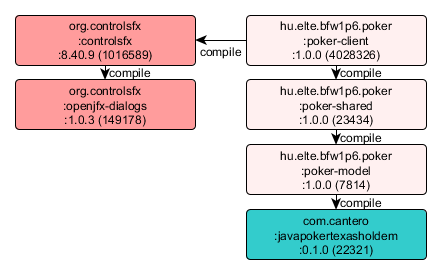
\includegraphics[width=11cm]{developer-documentation/images/poker-client-deps.png}
\end{figure}
\begin{figure}[h!]
	\caption{Szerver modulra bontása}
	\label{fig:server_modul}
	\centering
	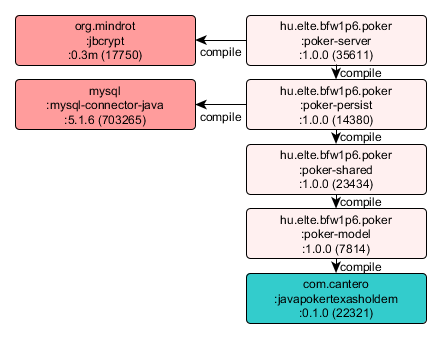
\includegraphics[width=11cm]{developer-documentation/images/poker-server-deps.png}
\end{figure}
A modulok közötti függőséget a \ref{fig:client_modul}. és a \ref{fig:server_modul}. ábra szemlélteti. \\
A programcsomag két főmodulra bontható
\begin{itemize}[leftmargin=2.7cm]
\item poker-server
\item poker-client
\end{itemize}

\subsection{Model modul} \label{sec:poker-model}
A poker-model modul felelős a játék modellezéséért. A \ref{fig:model} ábrán látható a modul felépítése. 
\begin{figure}[h!]
	\caption{A model felépítése}
	\label{fig:model}
	\centering
	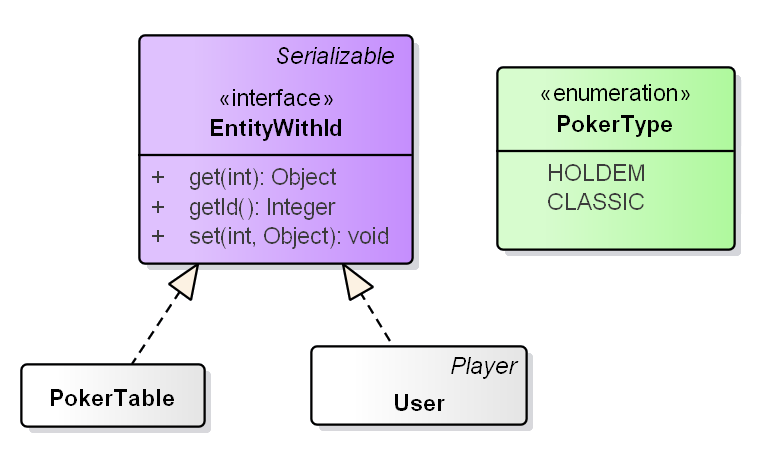
\includegraphics[width=11cm]{developer-documentation/images/model.png}
\end{figure}
Az entitásokat össze kellett fogni az \texttt{EntityWithId} interfész segítségével, ezáltal a DAO objektumot generikusan lehetett megfogalmazni, amely segített a kód duplikációk elkerülésében. A\texttt{PokerTable} és a \texttt{User} osztályok példányai feleltethetőek meg a \texttt{poker\_tables} és a \texttt{users} adattáblák egyes rekordjainak. A \texttt{PokerType} enumeráció a játékstílusokat határozza meg. Ha egy új játékstílust szeretnénk hozzáadni a játékhoz, akkor a kódban egy új \texttt{PokerType} enum objektumot kell felvennünk, és a \texttt{poker\_schema.sql} állományban pedig fel kell venni egy új insert utasítást a \texttt{poker\_types} táblára nézve az új játékstílus nevére vonatkozólag. Természetesen ez a pár sor újonnan hozzáadott kód nem azt jelenti, hogy már használhatjuk is az új játékstílust. A programcsomagot több ponton is ki kell bővíteni
\begin{itemize}[leftmargin=2cm]
	\item Szerver oldal
		\begin{enumerate}
			\item AbstractPokerTableServer osztályt ki kell terjeszteni egy új osztállyal
		\end{enumerate}
	\item Kliens oldal
		\begin{enumerate}
			\item Új leszármazott osztályokat kell létrehozni a kliens oldali MVC absztrakciós osztályaiból
			\item Új fxml állományt kell létrehozni
		\end{enumerate}
\end{itemize}

\subsection{Shared modul}
A poker-shared modul olyan közös osztályokat tartalmaz, amelyeket a kliens és a szerver egyaránt használ. Itt helyezkednek el az egyéni kivételek, a kommunikációs rendszer definíciója és a kliens, mint megfigyelő interfésze.

\pokerparagraph{Kivételek}
A játékcsomagnak szüksége van egyéni kivételekre. Az olyan speciális eseteket, mint például adabázisba írás, illetve abból olvasás közbeni fellépő kivételt saját kivételobjektumokkal célszerű lekezelni. Ehhez hasonló egyéni kivételek fellépthetnek például bejelentkezéskor, asztalhoz való csatlakozáskor, hibás jelszó megadás esetén.

\pokerparagraph{Kommunikációs rendszer}
A szerver és a kliens üzeneteket küldhetnek egymásnak. A kommunikációs rendszer viszonylag absztrakt módon került implemenetálásra ezzel is elősegítve a későbbi bővíthetőségi nehézségeket. Azonban sajnos helyenként fellelhető kód duplikáció az enumerációkra való építkezés miatt. \\
Minden utasításnak kötelezően implementálnia kell a \texttt{PokerCommand} interfészt, ezzel is elősegítve az általános megfogalmazást a rendszerben. Két fajta utasítás létezik a játékcsomagban:
\begin{itemize}[leftmargin=2cm]
	\item Szerver utasítás
	\item Kliens utasítás
\end{itemize}
Továbbá a játékstílusnak megfelelően tovább specializálódik a küldendő üzenet fajtája. A programcsomag kettő játékstílust fogalmaz meg \ref{subsubsec:game_styles}. A játékstílusok különböző utasítás fajtákat igényelnek. Értelemszerűen, ha egy Holdem játékstílusban résztvevő kliens üzenetet szeretne küldeni a játék asztal szervernek , akkor egy \texttt{HoldemPlayerCommand} típusú objektumot kell elküldenie a szerver csonkon keresztül.

\pokerparagraph{Observer pattern \cite{observer_pattern}}
Az oberserver tervezési minta segítségével megvalósítható RMI API-n keresztül az úgynevezett event driven server (magyarul kéne...?). Így nem csak a kliens tud üzenet küldeni a szervernek, hanem a szerver is tudja értesíteni a klienseket. Például, ha egy játékos játékstílustól függetlenül CHECK típusú utasítást küldött a szervernek, akkor azt az üzentet a szerver minden kliensnek szétszórja.

\pokerparagraph{Session}
% ez a szöveg lehet, hogy server modulba kéne....
A szerver a klienseket session objektumokkal azonosítja. Minden kliens kap egy sessiont a bejelentkezéskor. A session addig él, amíg a felhasználó ki nem jelentkezik, akkor ugyanis a munkamenet érvénytelenítésre kerül. Illetőleg a munkamenetet akkor is érvényteleníteni kell, ha a kliens nem jelentkezett ki, de a kapcsolat valamilyen oknál fogva megszakadt. \\
Amikor egy kliens be szeretne jelentkezni a játékba, akkor a szerver az összes megszakadt kapcsolatú klienst felderíti, és a munkamenetüket érvénytelennek tekinti. A felderítés úgynevezett pingeléssel történik. A szerver minden csatlakozott klienst megpróbál elérni, és amelyik kliensnél megszakadt a kapcsolat, azt eltávolítja a szerverről. Ezután a \texttt{SessionService} ellenőrzi, hogy az adott felhasználónévvel van-e aktív munkamenet, ha van, akkor kivételt dob az eljárás, különben az autentikáció sikeres, és a kliens oldali model eltárolja a loginkor kapott sessiont.

\subsection{Persist modul}
A poker-persist modul látja el az adatbázissal kapcsolatos teendőket. Ez a modul írja és olvassa az adatbázist a bejövő kérések és paraméterek alapján.

\pokerparagraph{Generikus DAO}
A generikusság elengedhetett a kódismétlés elkerülése végett. Általánosan kell megfogalmazni az entitások viselkedését \ref{sec:poker-model} és ezáltal a persist modul letisztult arculatot kap. A \texttt{GenericDAO} osztály tartalmaz minden olyan elemet, amelykre a specializálódott DAO-knak szükségük lehet.

\pokerparagraph{Adatbázis menedzser}
Az \texttt{AbstractDAO}-nak szükséges van tényleges adatbázis kapcsolatra, amelyet a \texttt{DBManager} osztály szolgáltat.

\pokerparagraph{Kivételek átfordítása}
Az \texttt{AbstractDAO} rendelkezik egy \texttt{SQLExceptionTranslator} objektummal is, amely az adatbázisból érkező hibát fordítja át \texttt{PokerDataBaseException} típusú kivételre. A \texttt{PokerDataBaseException} kivétel osztály a felhasználó számára is értelmes hibaszöveget hordoz magában.

\subsection{Kliens modul}
A kliens modult és annak minden függőségét egy jar fileba csomagolva kell szétterjeszteni a felhasználók között, akik majd ténylegesen használni fogják a programot. A \ref{fig:client_modul}. ábra alapján a jar file tartalmazni fog minden olyan osztályt és interfészt, amelyre ténylegesen szüksége lesz a kliens programnak. Az összecsomagoláshoz igénybe vehetjük a mavent és annak az assembly pluginját. A poker-client könyvtárban a
 \begin{verbatim}
mvn clean compile assembly:single
\end{verbatim}
paranccsot kiadva a \path{poker\release} könyvtár alá csomagolódik be a futtatható jar állomány.

\pokerparagraph{Model-View-Controller \cite{MVC}}
Az igen közkedvelt tervezési minta alapján valósítottam meg a kliens oldali programot.
%lol2
\pokerparagraph{Model}
A kliens kettő darab model osztályt tartalmaz. Az \texttt{Model} nevű singleton osztály felelős a szerver felé irányuló kapcsolat kiépítésében és fenntartásában. Ez az egyszerű szerver hívásokat végzi el. A kliens indulásakor elkéri az RMI registry-ből a szerver csonkot, és bejelentkezéskor eltárolja a szerver által generált munkamenet objektumot. A model segítségével hívhatóak meg a játék funkcióinak a zöme. Ide sorolható a játék minden olyan funkciója, amely nem játék asztalhoz köthető. Például ennek a modelnek a segítségével lehet bejelentkezni, asztalt és felhasználót módosítani, vagy akár a játékasztalokat elkérni a szervertől. \\
A kliens tartalmaz egy másik modelt - \texttt{AbstractMainGameModel} -, amely a tényleges játékért felel kliens oldalon. A szerver a parti megkezdésekor leküldi a klienseknek, hogy az adott partiban ki hol ül az asztalnál, hány játékos ül az asztalnál, a játékosok neveit és még néhány inicializációs értéket. Ezen értékek alapján a model el tudja dönteni, hogy az adott kliensnek kötelezően be kell rakni vakot. Minden parti elején minden kliensnek az adóssága a nagy vakkal egyezik meg. A további körökben az adósság leróható.

\pokerparagraph{View}
A megjelenítésért a JavaFX 2 \cite{javafx} felel. Az alapkonstrukció, hogy a GUI-n megjelenő objektumok zömét fxml állományokba szervezzük és a megjelenítés színtérgráffal történik. Minden fxml állományhoz pontosan egy controller tartozik, amely az fxml állomány minden újratöltésekor inicializálódik. A controllert az adott fxml állomány gyökerébe kell bekötni. \\
A programcsomag által definiált játékstílusok igen hasonlóak, ezért egy \texttt{AbstractMainView} osztályban megfelelően kiszervezhetőek a közös részek, majd ennek az osztálynak a specializációiban: \texttt{ClassicMainView}, \texttt{HoldemMainView} kerülnek megvalósításra a tényleges játékstílusbeli különbségek. Például eltérő különbség , amely a GUI-n is megjelenik, hogy a játékosok hány darab kártyalapot kapnak kézbe, illetve a Texas Hold'Em játékstílussal ellentétben a classic játékmódban nincsenek közös kártyalapok.

\pokerparagraph{Controller}
A controller általános szerepét ugyancsak egy absztrakt osztály, az \texttt{AbstractMainGameController} tölti be. A közös részek nem csak a megjelenítés és a model szintjén figyelhetőek meg, hanem az őket összekötő controller szintjén is. A beérkező utasítások alapján a controller hív tovább a megjelenítési és a model rétegbe.

\pokerparagraph{FrameController}
Alapvetőleg a vezérlő réteg objektumai között nincs egy egységes kapocs, amely összefogná őket. Az egyes vezérlő réteg objektumok nem ismernek más vezérlő rétegbeli objektumot, továbbá aktuálisan mindig pontosan egy controller van betöltve, így párhuzamosan sem futhatnak. Ez alól néhány controller kivételt képez. Ugyanakkor bizonyos esetekben szükség van más megjelenítési és vezérlési réteg betöltésére az éppen aktuálisan betöltött controller által. A \texttt{FrameController} eggyel magasabb absztrakciós szinten helyezkedik el, így oldva meg a fenti problémát. Amikor egy új vezérlő rétegbeli objektumot töltünk be, akkor az objektumnak át kell adni egy \texttt{FrameController} objektum példányt, mint amolyan delegált objektumot, amelynek segítségével az egyes controllerek ki tudják cserélni a megjelenítési és vezérlési réteget. Fontos megjegyezni, hogy a csere a model réteget nem érinti.

\pokerparagraph{CommunicatorController}
A szervernek értesíteni kell a klienseket az adott asztalnál történő eseményekről. A kliensek ennek elérése végett egy publikus interfészt biztosítanak és feliratkoznak a szerverhez. A szerver a kliensek beregisztrált objektumait nyilván tartja, és ezeken keresztül tudja értesíteni őket. A kliensek erre a feladatra egy külön objektumot - \texttt{CommunicatorController} - hoznak létre, és küldenek el a szerverhez. Az üzenetváltó objektumok az éppen betöltött kliens oldali vezérlő rétegbeli objektumot delegált objektumként konstruktori paraméterként kapják meg, így a szerver által küldött üzenetek fogadása után az üzeneteket tovább tudják küldeni a vezérlő rétegnek.

\pokerparagraph{PokerRemoteObserver}
Minden olyan kliens oldali vezérlői rétegbeli objektumnak implementálnia kell ezt az interfészt, amely működése során üzenetet fogad a szervertől, amelyet továbbít a kliens további rétegeinek.

\subsection{Szerver modul}
\begin{figure}[h!]
  \caption{A szerver publikus interfésze}
  \label{fig:server_public}
  \centering
    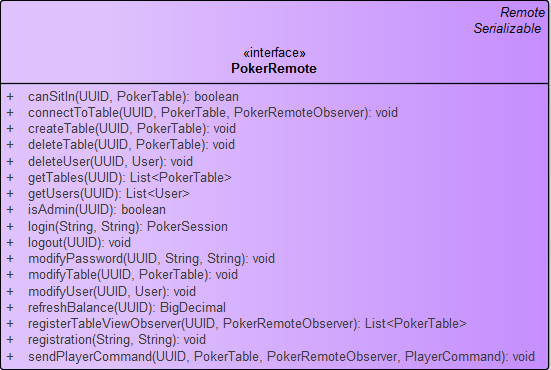
\includegraphics[width=\textwidth]{developer-documentation/images/server_remote.png}
\end{figure}
A szerver feladata a játék biztosítása a kliensek számára. A \ref{fig:server_public}. ábrán látható a szerver jóldefiniált publikus interfésze. A kliensek ezt az interfészt tudják elkérni az RMI registry-ből. A \texttt{PokerRemote} interfészt a \texttt{PokerRemoteImpl} osztály implementálja, ennek egy instanciája a tényleges szerver objektum. A szerveren futnak a játékasztal-szerverek, amelyek egy-egy asztalnak feleltethetőek meg, amelyekhez a kliensek csatlakozni tudnak. Ha egy játékos csatlakozik egy játékasztalhoz, akkor az adott asztal feljegyzi a csatlakozott klienst egy lokális listába. A főszervernek továbbra is van referenciája a klienshez, ugyanis minden klienstől érkező utasítást a főszerver fogad, és irányít a megfelelő játékasztal-szerverhez. Erre az autentikáció miatt van szükség. Azonban ez a fajta megközelítés könnyen szűk keresztmetszetté válhat \cite{bottleneck}. \\
A szerver a jelszavak titkosítására bcrypt \cite{bcrypt} eljárást alkalmaz, amelynek a biztonságát sózással növeli. Továbbá a szerver felhasznál még egy külső csomagot - mysql-connector-java -, amely az adatbázis kapcsolatért felel.

\subsection{javapokertexasholdem modul}
Külső könyvtár, amely eredetileg Texas Hold'Em játékstílusban tud kezeket kiértékelni. Az integrációt viszonylag könnyen meg lehetett oldani, ráadásul még általánosítani is sikerült a könyvtárat. Tehát classic és Texas Hold'Em játékstílusra is ugyanezt a könyvtárat használja a szerver a kezek kiértékelésére.

\section{Funkciók}
A szerver vázáért a PokerRemote interfész felel, amely a játékon végrehajtható műveletek összefogásáért felel. Itt található az összes funkció, amely megvalósításra került, mint például játék asztal létrehozása, új felhasználó létrehozás, admin jog kiosztása stb. A kliens ezt a vázat tudja elkérni az RMI registry-ből, mint kliens-oldali szervercsonk, amelyeken a műveletek meg tudja hívni.
\subsection{Általános funkciók}

\pokerparagraph{Regisztráció}
A játékot csak regisztrált felhasználók tudják használni. A szerver biztosít regisztrációs lehetőséget a felhasználók számára. A regisztráció során felhasználónevet és jelszót köteles megadni a felhasználó, amely tárolásra kerül az adatbázisban. Minden újonnan regisztrált felhasználó 1000 egységnyi egyenleggel rendelkezik. Az adatbázis séma nem engedi, hogy több azonos felhasználónévvel különböző felhasználók regisztrálva legyenek, erre a regisztráció során ügyelnie kell a felhasználónak.

\pokerparagraph{Bejelentkezés}
A játék használatához a játékosoknak be kell jelentkezniük. Egy felhasználónévvel egyidőben csak egy munkamenet létezhet. Ha a felhasználó már használatban lévő felhasználónévvel kíván beljelentkezni, akkor a szerver hibás bejelentkezési adatokra hivatkozva megtagadja az utasítást. Sikeres bejelentkezést követően a szerver példányosít egy PokerSerssion objektumot egy UUID \cite{uuid} azonosítóval, amelyet lokálisan eltárol, majd a kliensnek elküld. A kliens a kijelentkezésig megőrzi ezt az objektumot, és a későbbi funkciók hívása során ezzel a munkamenettel azonosítja magát.

\pokerparagraph{Kijelentkezés}
A játékosok a kijelentkezés funkcióval hagyhatják el a játékot. A funkció hivása során a kijelentkezni kívánó felhaszáló munkamenetét a szerver érvényteleníti, és a felhasználó visszakerül a bejelentkezési formhoz. A szerver (korlátozott mértékben) fel lett készítve a nem szabályszerű kijelentkezésre, tehát ha például megszakad a kapcsolat a klienssel, akkor a legközelebbi bejelentkezési funkció hívása során a szerver érvényteleníti a megszakadt kliensek munkameneteit, ezzel elérve azt, hogy a foglalt felhasználónevekkel újra be lehessen jelentkezni.

\pokerparagraph{Asztalok}
\pokerparagraph{Létrehozás}
A funkció eléréséhez admin jogosultságra van szükség. Egy új asztalt lehet lérehozni az adatbázis séma (hivatkozás) irányelvei szerint megfelelően paraméterezve. Amikor a kliens asztalt szeretne létrehozni, akkor a szerver egyértelműen tájékoztatja, hogy az asztal létrehozás sikeres volt-e. Ha igen, akkor egy felugró üzenet jelenik meg a képernyőn, hogy az asztal létrehozása sikeres volt, majd a felhasználó vissza lesz irányítva a tábla listázó felületre. Ha az asztal létrehozása sikertelen volt, akkor a felület ugyancsak egyértelműen jelzi a felhasználónak, hogy a művelet miért hiúsult meg. Például előfordulhat hibás beviteli érték, szerverhiba és adatbázishiba is.

\pokerparagraph{Módosítás}
Egy már meglévő asztalt adminisztrációs joggal rendelkező felhasználó módosíthat. Fontos megjegyezni, hogy a módosítás csak üres asztalokra alkalmazható.
\pokerparagraph{Törlés}
A funkcióhoz ismételten adminisztrációs jog szükséges. Már létező asztal törölhető a funkció segítségével. A funkciót csak üres asztalokra lehet alkalamazni.
\pokerparagraph{Lekérés}
A bejelentkezést követően a felhasználó a táblalistázó felületre kerül, ahol megtekintheti a létrehozott és elindított játéktábla-szervereket (hivatkozás). A bejelentkezést követően a kliens ezeket az asztalokat elkéri a szervertől. Fontos megjegyezni, hogy ha bármelyik asztal módosításra került, akkor az asztalokat a szerver újra leküldi a klienseknek, így minden kliensnél az asztalok legfrissebb változata lesz elérhető.

\pokerparagraph{Csatlakozás}
A felhasználók létrehozott játékasztal-szerverekhez csatlakozhatnak. Fontos megjegyezni, hogy egy asztalnál maximum 5 játékos ülhet egyszerre, tehát ha egy asztal tele van (5 játékos ül az asztalnál, beleszámolva a következő partira váró játékosokat is), akkor kliens oldali kód nem engedi beülni a felhasználót az adott asztalhoz, amelyről a felhasználót a képernyőn értesíti. Ha egy tele asztaltól kilép az egyik játékos (vagy megszakad a kommunikáció), akkor az asztalnál felszabadul egy hely, amelyet egy új felhasználó elfoglalhat, ekkor az asztal ismét tele lesz.

\pokerparagraph{Szabad helyek lekérdezése}
Ha egy kliens be szeretne ülni az egyik játékasztal-szerverhez, akkor előbb le kell kérdeznie, hogy van-e még szabad hely az asztalnál.

\pokerparagraph{Felhasználók}
\pokerparagraph{Létrehozás}
A regisztráció során új felhasználó entitás jön létre, amelyet a szerver letárol az adatbázisban. A funkció külön, direktbe nem hívható, regisztrációhoz kötött.

\pokerparagraph{Egyenleg visszaállítás}
A felhasználók egyenlegét adminisztrációs joggal rendelkező felhasználó vissza tudja állítani alaphelyzetbe, amely 1000 egységnek felel meg.

\pokerparagraph{Törlés}
Ugyancsak adminisztrációs jogot követel meg egy felhasználó végleges eltávolítása a póker játékból.

\pokerparagraph{Lekérés}
Az adminisztrációs joggal rendelkező felhasználók lekérdezhetik az adatbázisból az összes regisztrált felhasználót. A felhasználók a képernyőn táblázatos formában jelennek meg, amelyből felhasználót ki lehet választani a további funkciók eléréséhez.

\pokerparagraph{Jelszó csere}
A felhasználóknak lehetőségük van jelszócserére.

\pokerparagraph{Adminisztrációs jog}
A szerverre beregisztrált felhasználók alapesetben nem rendelkeznek ilyen jogosultsággal. Az adminisztrációs jogot csak adminisztrációs joggal rendelkező felhasználó tudja kiosztani illetve megvonni. Friss adatbázis esetén létezik egy admin nevű felhasználó, aki adminisztrációs joggal rendelkezik. Kezdetben csak ez a felhasználó tud kiosztani adminisztrációs jogot.

\subsection{Játékmenetbeli funkciók}
\pokerparagraph{Utasítás küldés}
A szerver és a kliens kommunikációja a programcsomag által definiált üzenetobjektumokkal történik. Bármilyen játékközbeni utasítást szeretne küldeni a kliens a szervernek, vagy éppenséggel a szerver a kliensnek, azt be kell csomagolnia egy \texttt{PokerCommand} interfészt implementáló osztályba. A szerver és a kliens parti közben csak ilyen típusú üzenetek fogadására alkalmas. Pontosabban fogalmazva az implementációs nehézségeken túllendülve a klienseket fel kellett készíteni arra, hogy a szerver adott esetben megpingelheti őket.

\pokerparagraph{Egyenleg lekérése}
A szerver az automatikus egyenleg frissítést nem támogatja. Az egyes klienseknek egyenként kell arról gondoskodniuk, hogy a grafikus felületen mindig az éppen aktuális egyenlege jelenjen meg a játékos számára.

\section{Tesztelés}
\subsection{Funkcionális tesztelés}
\begin{tabular}{| C{4.7cm} | C{4.7cm} | C{4.7cm} |}
\hline
  Funkció & Elvárt eredmény & Eredmény \\ \hline
  Regisztráció & A felhaszáló a regisztráció gomb megnyomása után tájékoztatást kapjon afelől, hogy a regisztráció sikeresen megtörtént. & A program az elvártnak megfelelően működött. \\ \hline
  Bejelentkezés & A bejelentkezési formot helyesen kitöltve és a bejelentkezés gombra kattintva a program sikeresen autentikálta és átirányította a felhasználót a táblalistázó felületre. & A program az elvártnak megfelelően működött  \\ \hline
  Játék asztalhoz való beülés egyedüli játékosként & Az asztal betöltődik és a felhasználó profilján kívül a grafikus interfészen más profilkép nem jelenik meg. Tetszőleges idő eltelte után sem indulhat el a játék, kivétel ha legalább egy másik felhasználó csatlakozik az adott játék asztalhoz  & A program az elvártnak megfelelően működött. \\ \hline
  Játék asztalhoz való beülés nem egyedüli játékosként & Ha az asztalnál éppen parti zajlik, akkor ebből az újonnan csatlakozott játékos semmit nem érzékel. A játékos a következő partiba szállhat be. A következő parti megkezdődik, ha legalább kettő darab játékos ül az asztalnál. & A program az elvártnak megfelelően működött. \\ \hline
  Tábla módosítás & - & - \\ \hline
  Tábla törlés & - & - \\ \hline
\end{tabular}

\section{Tovább fejlesztési lehetőségek}
\begin{itemize}
\item Az adatbázis viszonylag alacsony absztrakciós szinten került implementására, azonban mivel néhány tábláról beszélhetünk csak, ezért igyekeztem elkerülni a keretrendszerek általi overheadet. Ugyanakkor ezen a ponton sokat fejlődhet a programcsomag, ha a későbbiek során esetlegesen bonyolultabban kellene modellezni a játékot adatbázis szempontjából. Például dialektusok - akár Liquibase (hivatkozás) - használata elfedheti a tényleges adatbázis-kezelő rendszer általánosságait, így eggyel magasabb szintre helyezhető a megvalósítás.
\item A felhasználói élményen sokat javíthat az animációk használata. A megjelenítés sokkal lágyabb, folyékonyabb lehetne Transition/Animation (bibliográfiába hivatkozás...) objektumok használatával.
\item Akár a komplett RMI architektúrát le lehetne váltani, és helyette REST szoftverarchitektúrát alkalmazni, amely modernebb megjelenést (AngularJS, reszponzív design) és modernebb fejlesztői eszközöket, API-kat vonna maga után.
\item A játék nem képes kezelni olyan eseteket, amikor egynél több játékos nyer az adott körben.
\item A játék nincs felkészítve arra a szélsőséges esetre, ha valakinek elfogy a zsetonja, akkor pontosan minek (és hogyan) kell történnie.
\item A kódban viszonylag sok kód duplikáció van jelen, ugyanis az HouseCommandType és a PlayerCommandType enum típusú objektumok szűk keresztmetszetnek tudható be. Ha a PokerCommand interfacet implementáló osztályokat generikusan tudnánk megfogalmazni, akkor jelentősen letisztulna a kód.
\item Az admin jogot el lehetne távolítani a játékból, és helyette MVC tervezési minta alapján a szerver oldalra is implementálni lehetne egy grafikus interfészt, amelyen keresztül a szerver teljeskörű karbantartása és adminisztrációja elvégezhető lenne.
\item A programcsomag a váratlan adatbázis hibákat nem tudja megfelelően lekezelni. Ezek javításra szorulnak.
\item A programcsomag szerver oldali kódja a konkurens helyzeteket nem mindig kezeli le helyesen. Például ha egy játékasztalhoz a kliensek gyorsan fel-lecsatlakoznak. Ebből fakadóan előfordulnak bugok és szükség volt kliens oldalon és szerver oldalon is egy-egy mentőövet implementálni. Kliens oldalon a Q betű segíti a felhasználókat a hibás játékasztal elhagyásában, szerver oldalon pedig egy reset nevű metódus került implementálásra, amit adminisztrációs joggal lehet meghívni.
\end{itemize}


\clearpage
